\documentclass{deliverablereport}
\usepackage{textcomp}

\deliverable{dissem}{press-release-2}
\deliverydate{16/12/2019}
\duedate{31/08/2019 (M48)}
\author{Izabela Faguet, Viviane Pons, Nicolas M. Thiéry}

\begin{document}
\maketitle
% This will be the abstract, fetched from the github description
\githubissuedescription

% write the report here

\section{End of project press releases}

During the first months of the project we had published six press
releases and we had planned to do the same at the end to promote the
actions and the results by providing targeted information to broad
audience (including the media and the public).


The press releases are the result of a joint effort of the partners,
which followed our usual open bottom up approach.

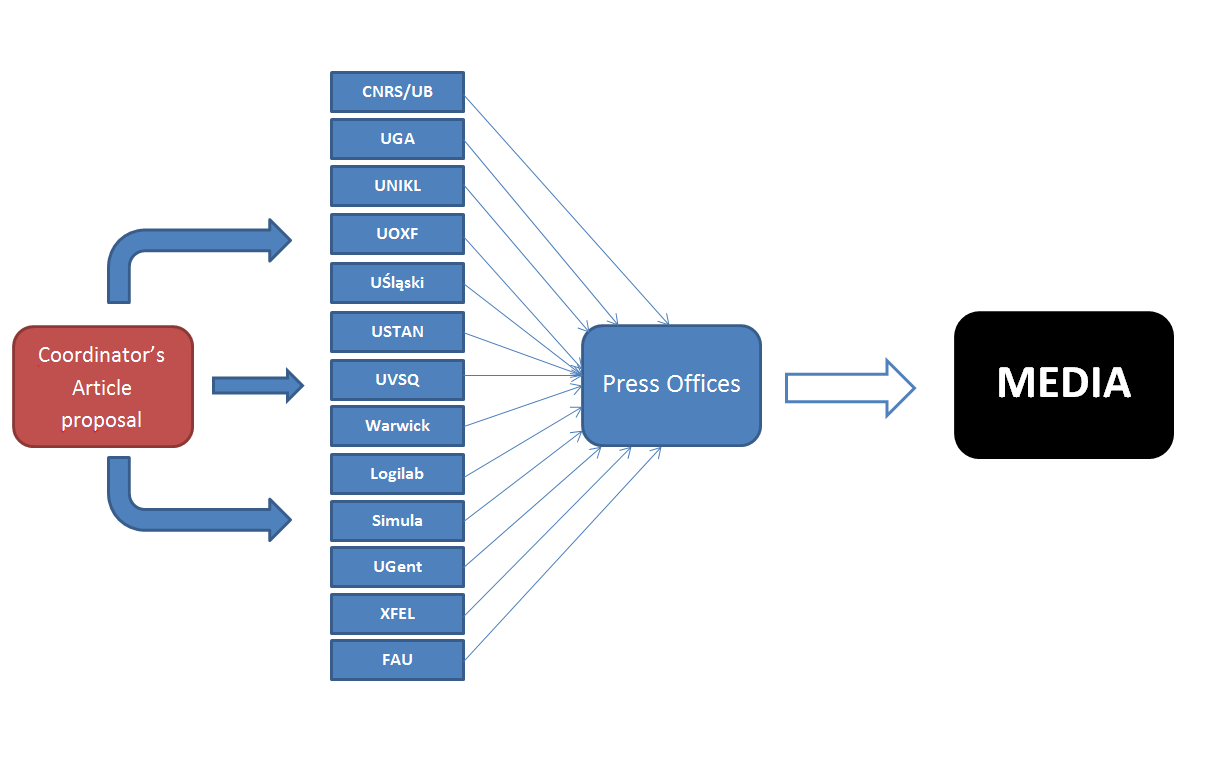
\includegraphics[width=\textwidth]{PressReleasesProcess.png}

Some of the beneficiaries, including the coordinator, reached to their
Press Office to inquire about adequate forms and processes. Based on
our Summary for Publication, UPSud's Press Office proposed a quick
draft in French as source of inspiration. The coordinator then lead
the collective writing of a general joint text. This text served as
template that each beneficiary could adapt to suit its own
circumstances and translate into the local language as required. The
produced press releases were then circulated to the respective press
or communication offices, which should lead to about twelve releases.

% , leading to at least 12 releases in general press in the high
% education, research area, and local press.

\section{End of project communication through OpenDreamKit's channels}

OpenDreamKit's website (\url{https://opendreamkit.org/}) served as a
major dissemination tool in terms of project’s concept, objectives and
outcomes. It provides information on the project content, objectives,
partners, planned activities, events organized within the project and
deliverables. It's complemented by a
\href{https://twitter.com/OpenDreamKit}{@OpenDreamKit} Twitter
account, and a video channel. Both serve as direct communication
instrument to reach the general public and interact with other
communities such as GAP, SageMath, Cocalc, or Jupyter.

During the project, seven video interviews were created to communicate
about the project, its main goals and the consortium to a wider
public; and 3 explainer videos that tell the story of our project in a
way understandable for a non scientific public. The videos will be
used across online platforms, and promoted through the project’s
online communications channels such as YouTube. A Youtube account for
OpenDreamKit project was set up to host the video series. The number
of views, and comments for each video were monitored as KPIs in the
technical report.

On the day after the final review meeting, we published a
\href{https://opendreamkit.org/2019/10/30/final-project-review/}{blog post}
on our website highlighting our presentations and the assessment made
by the referees and the Project Officers.

An overview of the project outcomes was produced by UPSud with the
technical contribution of the ODK partners (see appendix B), and
will be published on OpenDreamKit's web site; it takes the form of an
extended version of the Summary for Publication produced at the
occasion the last reporting period. It complements the press release
by being more detailed on the concrete actions and the impact on end
users, with link to related material (reports, blog posts, ...). Soon
after its publication, a blog about the future of OpenDreamKit
community will posted, and both will be advertised through social
media (twitter, ...). We also plan to launch targeted email campaigns
in order to reach to our scientific communities about the significant
developments on ODK project activities and results.


% In order to reach a broad target, the presence of the ODK project in social media was
% also encouraged. 

% The website will have direct access to these social networks by clicking over the icon 
% situated on a visible part of the website. In this way, it will be easy for every user 
% to participate in this when the website is visited.

\section{End of project communication through the European Commission's channels}

The Coordinator has contacted the communication officer  who will support the dissemination
of the results of the project ad will promote them through the EC's communication channels. 
The communication officer will publish an article and a presentation of the project in the 
newsletter “Digital Excellence \& Science Infrastructure” of the European Commission, 
on the European Commission website \url{https://ec.europa.eu/digital-single-market/} to reach 
a wider audience, potentiating its outreach. 
HORIZON, the EU Research \& Innovation e-magazine, will also be used to inform about 
the benefits and progress that ODK will generate in Europe, informing about 
the open debates created and the results.
The Coordinator has also been contacted by a journalist who works for CORDIS' Editorial
 Services consortium Tipik/Intrasoft International. OpenDreamKit was chosen from among 120
projects selected monthly, based on domain, timing and quality of results by the CORDIS magazine Team
to feature highlights and results from the most exciting EU-funded research and development projects.
Our work will be promoted on the CORDIS website where it will be translated into multiple
languages and may be reused in the CORDIS magazine. In this communication strategy, we will
be sure to create an appropriate approach for the different audiences (policy makers, media,
general public, etc).

\clearpage
\appendix
\section{Press release template}

OpenDreamKit – Open-source development and community building in computational mathematics

Mechanising calculations has always been at the heart of mathematics, for exploring and discovering new mathematics,
even proving theorems. Beyond mathematics, computing has been and will ever more be a major driver of scientific progress. 
Thus, ever since the advent of the first machines, computing has been adopted as a tool of choice by mathematicians. 
It has become their microscope, and is used at all stages of their research.

In the last decades, vibrant communities of mathematicians have spearheaded the Open Science movement, developing a 
wide ecosystem of open tools covering all aspects of mechanized mathematics. The ecosystem suffered however from 
fragmentation and from lack of recognition: funding and career paths reward novel results rather than the daily work 
of fixing bugs and supporting users.

Meanwhile, early Virtual Research Environments (VRE) had proven their potential to better serve the growing needs of
mathematicians, reduce entry barriers, broaden the audience, and promote collaboration and Open Science. Hence, when 
the EU H2020 Research E-Infrastructure Program made a call for proposals centered on Virtual Research Environments, a 
few pioneers initiated an open process to bring these communities together and collectively craft an ambitious 7.6M€ 
research and innovation project, OpenDreamKit (opendreamkit.org). Coordinated by scientists from the Laboratoire de 
Recherche en Informatique (Université Paris-Sud and CNRS), OpenDreamKit involved 50 people spread over seven European
 countries: France, Belgium, Norway, Germany, Poland, Switzerland, United Kingdom; from 2015 to 2019, it employed an 
average of 11 full-time researchers and Research Software Engineers.

The existing ecosystem offered the potential to cover a large area of pure mathematics, and a variety of use cases 
ranging from a one-system one-laptop to multi-system institution-wide cloud deployments. This could not, however, 
be covered by a single one-size-fits-all VRE. Therefore, the objective was set instead to deliver a flexible toolkit
enabling research groups to set up Virtual Research Environments, customised to meet the varied needs of collaborative 
research projects in pure mathematics and applications, and supporting the full research life-cycle from exploration, 
through proof and publication, to archival and sharing of data and code.

To achieve this ambitious objective, OpenDreamKit built upon and contributed back to popular tools such as LinBox, MPIR, 
SageMath, GAP, PARI/GP, LMFDB, Singular, and MathHub, fostering ease of access and use, interoperability, and sustainability. 
It further joined forces with the general-purpose interactive computing environment Jupyter; in addition to outsourcing the 
user interface and VRE specific aspects, this maximised the impact on the scientific community at large.

OpenDreamKit gave new evidence of what can be achieved with proper support, especially through the work of Research 
Software Engineers. Thanks to them, some problems were solved which had been holding back the community for years, 
like bringing to fruition the effort to make the GAP software multi-threaded or porting the SageMath software and 
its dependencies to Windows.

Eventually OpenDreamKit was highly praised by its reviewers from the EU commission; hopefully this recognition 
can be used as leverage for future funding. Indeed, 

\textbf{The major challenge to come is to secure employment of a number of Research Software Engineers, as much as possible
 in long term positions, to support hundreds of contributors and tens if not hundreds of thousands of users of open-source 
mathematical software.}

\textbf{It is crucial as well to keep funding Jupyter core development: with millions of users, in academia and industry,
 Jupyter has become a key technology to support Open Science.}

One key of the success of OpenDreamKit was its ability to develop and sustain an active network of users and developers. 
Within the four years of the project, the group has built on their strong community building philosophy, especially through 
the organization of technical and educational workshops all over the world while actively promoting diversity. They organized
 over 80 workshops in about 20 different countries, including in developing countries, as with the first SageMath workshop 
in Nigeria. Some of these events were targeted more specifically at women, like the Women in Sage events in 2017 and 2019,
 to counter the wide gender gap in this field.

More generally, OpenDreamKit has been an occasion to promote a scientific development model based on openness, community,
 and shared technology. Beyond the traditional tentpoles of Open Science; namely Open Source, Open Data, and Open Publications;
 we have explored a novel concept, namely Open EU Project Management, and demonstrated its effectiveness. Indeed, we strongly
 believe that preparing the proposal and running the project completely in the open with a bottom up approach has played a 
fundamental role in engaging the communities, developing reciprocal trust, locating the toughest hurdles that users and 
developers actually face, co-designing solutions and co-implementing them efficiently.

\textbf{We strongly recommend the experience; long live OpenDreamKit’s spirit!}

\clearpage
\section{Summary for Publication (extended)}

\subsection{Summary of the context and overall objectives of the project (including the conclusions of the action)}

Automating calculations has always been at the heart of mathematics, for exploring and discovering new mathematics, even proving theorems. Beyond mathematics it has been and will play ever increasing role in scientific progress.

Thus, since the advent of first machines, computing was adopted as a tool of choice by mathematicians. It has become their microscope, and is used nowadays at all stages of their research.

Building that microscope takes dedicated and expert efforts! In the last decades, vibrant communities of mathematicians have spearheaded the Open Science movement, developing a wide ecosystem of open tools covering all aspects of mechanized mathematics: computation, tabulation (data), deduction, and narration. Today there are a hundreds of these, often highly optimized for specific domains such as solving differential equations, generating combinatorial objects like graphs or error-correcting codes, or classifying elliptic curves, objects with important implications on both Fermat's Last Theorem and cryptography.
 
The ecosystem suffered, however, from fragmentation and from lack of recognition, as funding and career paths reward novel results rather than the daily work of fixing bugs and supporting users; this led to long standing technical issues which impeded its sustainability in a rapidly evolving landscape of computing. 

Meanwhile early Virtual Research Environments (VRE) had proven their potential to better serve the growing needs of mathematicians, reduce entry barriers, broaden the audience, and promote collaboration and Open Science.

Hence, when the EU H2020 Research E-Infrastructure Programme made a call for  proposals centered on Virtual Research Environments, a few pioneers initiated an open process to bring the communities together and craft collectively a proposal.

The ecosystem offered the potential to cover a large area of pure mathematics, and a variety of use cases ranging from one-system-one-laptop to multi-system institution-wide cloud deployments. This could not however be covered by a single one-size-fits-all VRE.

Therefore, the aim was set to *deliver a flexible toolkit enabling research groups to set up Virtual Research Environments, customised to meet the varied needs of collaborative research projects in pure mathematics and applications, and supporting the full research life-cycle from exploration, through proof and publication, to archival and sharing of data and code*

To make this ambitious aim possible, the existing communities joined forces to build upon and contribute back to their tools -- in particular popular ones such as LinBox, MPIR, SageMath, GAP, PARI/GP, LMFDB, Singular, MathHub. They further joined forces with the general purpose interactive computing environment Jupyter; in addition to outsourcing the user interface and VRE specific aspects, this maximised the impact on the scientific community at large.

This was the birth of OpenDreamKit (\#676541), a 7.6M\euro project that, from 2015 to 2019, gathered 50 scientists spread over seven European countries: France, Belgium, Norway, Germany, Poland, Switzerland, and United Kingdom. Coordinated by the Laboratoire de Recherche en Informatique (Université Paris Sud and CNRS), OpenDreamKit employed an average of 11 full-time researchers and Research Software Engineers.

\subsection{Work performed from the beginning of the project to the end of the period covered by the report and main results achieved so far (including an overview of the results and their usage and dissemination)}

Over the duration of the project, work was performed on many fronts, in close collaboration with the community. 

One of the major hindrances for both end users and developers was limited availability and interoperability of various components of OpenDreamKit in different environments: oftentimes, software would work in the developers' environment (mostly Unix systems on Intel architectures), but fail in other environments (notably, Windows systems).

By integrating or updating best practices (continuous integration, continuous testing, ...), embracing emerging technologies (Docker containers, Conda packages, ...), by decoupling components and sharing infrastructure, we managed to make OpenDreamKit components available and interoperable in a much wider range of environments.  Notable success stories are:

\begin{itemize}
\item Porting of the components to Windows, MacOS and Linux;
\item Distribution of the components through official package repositories for major Linux distributions (Debian, Ubunut, Fedora, Arch, Gentoo);
\item Distribution of Docker images and Conda packages suited for deployment of our components in cloud environments (in particular, with JupyterHub and Binder integration);
\item Porting of SageMath to Python 3.
\item Modularization of various OpenDreamKit components, in particular SageMath and GAP.
\end{itemize}

To address the increasing need in high performance computing in computational mathematics, we drove the leading software components into supporting a large range of parallel architectures, from the low level SIMD, to GPUs, multi-core or clusters. Thanks to the introduction of new algorithms, tuned implementations and the design of parallel engines allowing to smoothly transition between various parallel settings, we made users able to harness the power of most modern computing platforms ranging from personal laptops to HPC clusters.

We contributed to a tight integration of OpenDreamKit components with Jupyter and to the Jupyter ecosystem itself, notably through new tools for collaboration (nbdime), validation (nbval), interactive web pages (thebelab), 3D visualisation (K3D-jupyter), interactive mathematics (sage-combinat-widgets, francy, ...), and through contributions to existing tools for collaborative workspace management (JupyterHub, JupyterLab). We also were early adopters, deployers and promoters of emerging technologies like Binder.

To demonstrate the applicability of our technology well beyond mathematics, we integrated micromagnetism computational engines into Jupyter to deliver a Virtual Research Environment taylored for interactive micromagnetism calculations.

We also authored four interactive textbooks, delivered numerous courses or actively helped colleagues doing so, in a variety of fields ranging from biology to computer science, all using Jupyter technology.

Finally we explored novel knowledge-based approaches for the high-level integration of large stacks of mathematical components. Like an interpreter for human language, it ensures meaning-preserving communication in mathematical languages between computation systems, databases, and humans. Concrete outcomes for bridging the gap between computation and data are already in production: data generation (py-persist/Memoize), online data exploration (data.mathhub.info) and live data exploration (sage-explorer).

All the outcome of the project were open and distributed widely through the usual channels to their target communities, reaching TRL 6 to 8. In addition, community building, training, and dissemination activities have been at the forefront of OpenDreamKit, with more than one hundred events organized or co-organized by OpenDreamKit, including developer workshops, training conferences, or satellite sessions, adding up to 1800 trainees. We also actively promoted diversity, through dedicated actions aimed at women and residents of developing countries. In particular, we organized two Women In Sage workshops and participated in or co-organized events in Colombia, Mexico, Nigeria, Algeria, Morocco, Tunisia, Palestine and Lebanon. We also created resources for researchers and teachers to accompany them in their use of the technologies we promote, such as tutorials, explainer comics and short videos. This includes contributions to the open textbook Computational Mathematics with SageMath which is nowadays reaching 500 downloads per day.

\subsection{Progress beyond the state of the art, expected results until the end of the project and potential impacts (including the socio-economic impact and the wider societal implications of the project)}

On the user-visible front, researchers, teachers and scientists in general now benefit from a rich uniform web-based user interface to all the OpenDreamKit computational components (from SageMath to C++!), which they can use on a wide variety of platforms, including tablet PCs, laptops, computer labs, all the way to cloud deployment and services, non-commercial (University-wide, EGI, Binder, ...) or commercial (Cocalc, Azure, OVH, Google, ...). We contributed to the deployment of a number of such installations for Mathematics, Computer Science, or Micromagnetism, demonstrating the versatility of the toolkit.

We have ourselves used extensively all the elements of the OpenDreamKit toolkit, while pursuing our own research, and while delivering many courses and training sessions in a wide variety of contexts --- from universities all over Europe, all the way to Nigeria or the AIMS institute in South Africa, creating interactive teaching material, sharing research results with the community, developing mathematical experiments, and much more.
This was the occasion to reflect on the adequacy and adoption of the tools for end-users, and immediately feedback the outcome into the project development.

By enabling Research Software Engineers to focus full time for months in a row on delicate challenges, we have tackled problems that the communities had been facing for a decade, such as bringing to fruition the effort to make GAP multi-threaded (HPC-GAP project) or porting SageMath and its dependencies to the Windows platform.
This has demonstrated the enormous value that Research Software Engineers (RSE) can bring to research, to support of end-users and collaborative developments by the community, and, generally speaking, Open Science. We have played an important role in the RSE movement, notably in the UK, exploring numerous hot and difficult questions: role, funding patterns, structuring, career paths, etc.

As was hoped, OpenDreamKit delivered a boost to the landscape of open source math software; it strives ever more than five years ago. We are particularly proud to have brought together many computational mathematics communities that, at earlier times, had been evolving independently, if not outright in a mostly counter-productive competition. Despite the occasional and unavoidable frictions occuring whenever needs and goals do not align, seeking collaboration has become the norm. 

\textbf{Nevertheless, the major challenge to come is to secure employment of a number of Research Software Engineers, as much as possible in long term positions, to support hundreds of contributors and tens if not hundreds of thousands of users of open source math software.}


As witnessed by the ACM award and by the wide adoption of the Jupyter technology in research, education (even at high school level), and industry, the Jupyter ecosystem has been booming during the course of OpenDreamKit; it is there to remain a major player of the field for years to come.  OpenDreamKit played a significant accelerator role by providing core Jupyter development.

Of particular relevance is its adoption by a number of EU-funded projects working towards the European Open Science Cloud (EOSC) -- in particular for remote access, remote analysis and visualisation of data, and for improved reproducibility. These projects directly benefit from outcomes of OpenDreamKit; they however position themselves as users of the Jupyter technology, not developers.

\textbf{It is therefore crucial that the EU keeps funding core Jupyter development, as an asset for the EOSC, science and industry, as well as to enable the continuing acceleration, and steering in the right direction, of this key open technology.}

Finally, beyond the traditional items of Open Science, namely Open Source, Open Data, and Open Publications, we have explored a novel item, namely Open EU Project Management, and demonstrated its effectiveness. Indeed, we strongly believe that preparing the proposal and running the project completely in the open with a bottom up approach has played a fundamental role in engaging the communities, developing reciprocal trust, locating the toughest hurdles that users and developers actually face, co-designing solutions and co-implementing them efficiently. 

\textbf{We strongly recommend the experience; long live OpenDreamKit's spirit!}


\end{document}

%%% Local Variables:
%%% mode: latex
%%% TeX-master: t
%%% End:
